\documentclass{beamer}
\usepackage{listings}
\usepackage{hyperref}
\usepackage{tikz}
\usetikzlibrary{positioning,shadows,arrows,shapes,calc}
\def\labelenumi\theenumi
\usepackage{graphicx}
\usepackage{amsmath}
\mode<presentation>{\usetheme{Frankfurt}}
\AtBeginSection
{
  \begin{frame}<beamer>
    \frametitle{Outline}
    \tableofcontents[currentsection,currentsubsection]
  \end{frame}
}
\title{Lecture 3: Barycentric Coordinates and Image Interpolation}
\author{Mark Hasegawa-Johnson}
\date{ECE 417: Multimedia Signal Processing, Fall 2023}  
\institute{University of Illinois}
\titlegraphic{\includegraphics{exp/block-I-primary.png}}
\begin{document}

% Title
\begin{frame}
  \maketitle
\end{frame}

% Title
\begin{frame}
  \tableofcontents
\end{frame}

%%%%%%%%%%%%%%%%%%%%%%%%%%%%%%%%%%%%%%%%%%%%%%%%%%%%%%%%%
\section{Application: Animating a still image}
\setcounter{subsection}{1}

\begin{frame}
  \frametitle{Input: X-Ray Microbeam Data}
  \centerline{\animategraphics[loop,controls,height=2.5in]{20}{exp/mp1_xrmb_movie-}{0}{47}}
\end{frame}

\begin{frame}
  \frametitle{Input: A Still Image Acquired Using MRI}
  \centerline{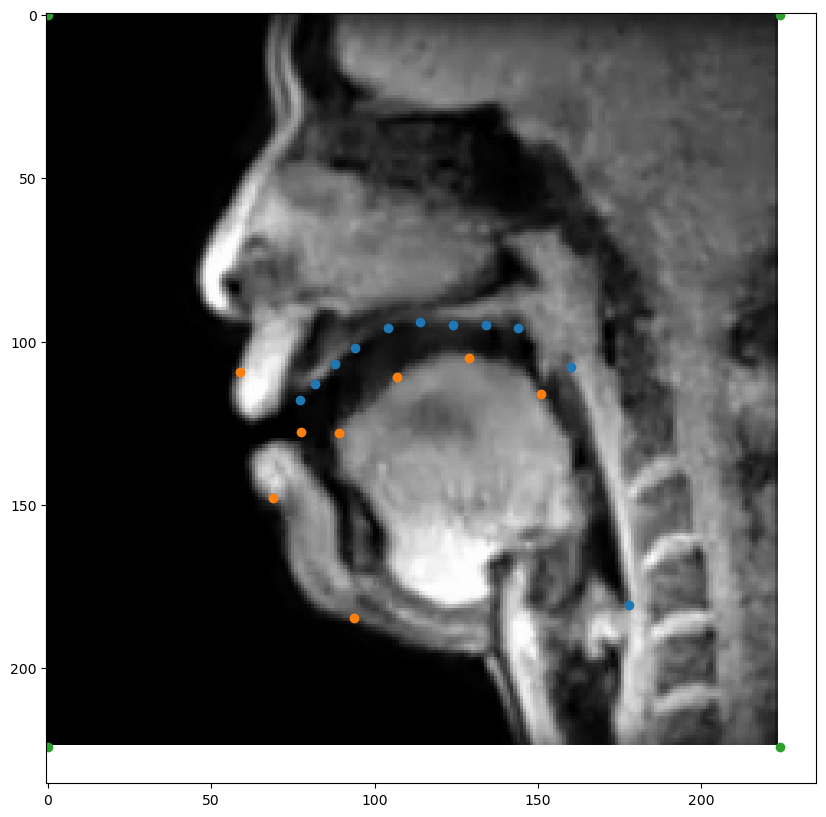
\includegraphics[height=2.5in]{mp1_mri_points.png}}
\end{frame}

\begin{frame}
  \frametitle{Desired Output: Animated Image}
  \centerline{\animategraphics[loop,controls,height=2.5in]{20}{exp/mp1_result-}{0}{47}}
\end{frame}

\begin{frame}
  \frametitle{Strategy}
  \begin{enumerate}
  \item Use affine projection to rotate, scale, and shear the XRMB
    points so that they match the shape of the MRI as well as possible.
  \item Draw triangles on the MRI so that every pixel is inside a triangle.
  \item Move the triangles.
  \end{enumerate}
\end{frame}

\begin{frame}
  \frametitle{Step 1 (Last time): Use affine projection to map XRMB to MRI}
  \centerline{\animategraphics[loop,controls,height=2.5in]{20}{exp/mp1_procrustes_movie-}{0}{47}}
\end{frame}

\begin{frame}
  \frametitle{Step 2 (Today): Draw triangles on the MRI}
  \centerline{\animategraphics[loop,controls,height=2.5in]{20}{exp/mp1_procrustes_triangles-}{0}{47}}
\end{frame}

%%%%%%%%%%%%%%%%%%%%%%%%%%%%%%%%%%%%%%%%%%%%%%%%%%%%%%%%%
\section{Barycentric Coordinates}
\setcounter{subsection}{1}

\begin{frame}
  \centerline{\href{https://www.youtube.com/watch?v=il6Z5LCykZk}{\includegraphics[width=4.5in]{../../../17fall/lectures/youtube_affine.png}}}
\end{frame}

\begin{frame}
  \frametitle{Piece-wise affine transform}
  \begin{itemize}
    \item OK, so somebody's given us a lot of points, arranged like
      this in little triangles.
    \item We know that we want a DIFFERENT AFFINE TRANSFORM for EACH
      TRIANGLE.  For the $k^{\textrm{th}}$ triangle, we want to have
      \[
      A_k = \left[\begin{array}{ccc}a_k&b_k&c_k\\d_k&e_k&f_k\\0&0&1\end{array}\right]
      \]
  \end{itemize}
  \centerline{\includegraphics[height=1in]{../../../17fall/lectures/mp7_image006.jpg}}
\end{frame}

\begin{frame}
  \frametitle{Piece-wise affine transform}
  \[
  \mbox{output point:}~\vec{x}=\left[\begin{array}{c}x\\y\\1\end{array}\right],~~~
  \mbox{input point:}~\vec{u}=\left[\begin{array}{c}u\\v\\1\end{array}\right]
  \]
  {\bf Definition}: if $\vec{x}$ is in the $k^{\textrm{th}}$ triangle in the
  {\bf output image}, then we want to use the $k^{\textrm{th}}$ affine transform:
  \[
  \vec{x}=A_k \vec{u},~~~\vec{u}=A_k^{-1}\vec{x}
  \]
  \centerline{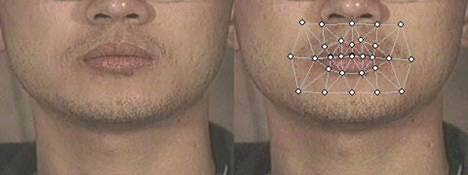
\includegraphics[height=1in]{mp7_image_warping_points.jpg}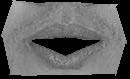
\includegraphics[height=1in]{mp7_image_warped.jpg}}
\end{frame}

\begin{frame}
  If {\bf it is known that} $\vec{u}=A_k^{-1}\vec{x}$ for some unknown
  affine transform matrix $A_k$,
  \vspace*{2mm}\\
  then
  \vspace*{2mm}\\
  the method of barycentric
  coordinates finds $\vec{u}$
  \vspace*{2mm}\\
  {\bf without ever finding} $A_k$.
\end{frame}

\begin{frame}
  \begin{columns}[t]
    \column{2.5in}
    \begin{block}{Barycentric Coordinates}
    Barycentric coordinates turns the problem on its head.  Suppose
    $\vec{x}$ is in a triangle with corners at $\vec{x}_1$,
    $\vec{x}_2$, and $\vec{x}_3$. That means that
    \[
    \vec{x}=\lambda_1\vec{x}_1+\lambda_2\vec{x}_2+\lambda_3\vec{x}_3
    \]
    where
    \[
    0\le\lambda_1,\lambda_2,\lambda_3\le 1
    \]
    and
    \[
    \lambda_1+\lambda_2+\lambda_3=1
    \]
    \end{block}
    \column{2.25in}
    \begin{block}{}
      \centerline{\includegraphics[width=2.25in]{../../../17fall/lectures/480px-TriangleBarycentricCoordinates.png}}
    \end{block}
  \end{columns}
\end{frame}

\begin{frame}
  \frametitle{Barycentric Coordinates}
  Suppose that all three of the corners are 
  transformed by some affine transform $A$, thus
  \[
  \vec{u}_1=A\vec{x}_1,~~
  \vec{u}_2=A\vec{x}_2,~~
  \vec{u}_3=A\vec{x}_3
  \]
  Then if
  \[
  \mbox{If:}~\vec{x}=\lambda_1\vec{x}_1+\lambda_2\vec{x}_2+\lambda_3\vec{x}_3
  \]
  Then:
  \begin{eqnarray*}
    \vec{u} &=& A\vec{x}\\
    &=& \lambda_1A\vec{x}_1+\lambda_2A\vec{x}_2+\lambda_3A\vec{x}_3\\
    &=& \lambda_1\vec{u}_1+\lambda_2\vec{u}_2+\lambda_3\vec{u}_3
  \end{eqnarray*}
  In other words, once we know the $\lambda$'s, we no longer need to
  find $A$.  We only need to know where the corners of the triangle
  have moved.
\end{frame}

\begin{frame}
  \begin{columns}[t]
    \column{2.5in}
    \begin{block}{Barycentric Coordinates}
      If
      \[
      \vec{x}=\lambda_1\vec{x}_1+\lambda_2\vec{x}_2+\lambda_3\vec{x}_3
      \]
      Then
      \[
      \vec{u}= \lambda_1\vec{u}_1+\lambda_2\vec{u}_2+\lambda_3\vec{u}_3
      \]
    \end{block}
    \column{2.25in}
    \begin{block}{}
      \centerline{\includegraphics[width=2.25in]{../../../17fall/lectures/480px-TriangleBarycentricCoordinates.png}}
    \end{block}
  \end{columns}
\end{frame}

\begin{frame}
  \frametitle{How to find Barycentric Coordinates}
  But how do you find $\lambda_1$, $\lambda_2$, and $\lambda_3$?
  \[
  \left[\begin{array}{c}x\\y\\1\end{array}\right]=
  \lambda_1\vec{x}_1+\lambda_2\vec{x}_2+\lambda_3\vec{x}_3
  =\left[\begin{array}{ccc}x_1&x_2&x_3\\y_1&y_2&y_3\\1&1&1\end{array}\right]
  \left[\begin{array}{c}\lambda_1\\\lambda_2\\\lambda_3\end{array}\right]
  \]
  Write this as:
  \[
  \vec{x}=X\vec\lambda
  \]
  Therefore
  \[
  \vec\lambda = X^{-1}\vec{x}
  \]
  This {\bf always works:} the matrix $X$ is always invertible, unless
  all three of the points $\vec{x}_1$, $\vec{x}_2$, and $\vec{x}_3$
  are on a straight line.
\end{frame}
\begin{frame}
  \frametitle{How do you find out which triangle
    the point is in?}
  \begin{itemize}
  \item Suppose we have $K$ different triangles, each of which is
    characterized by a $3\times 3$ matrix of its corners
    \[
    X_k = \left[\vec{x}_{1,k},\vec{x}_{2,k},\vec{x}_{3,k}\right]
    \]
    where $\vec{x}_{m,k}$ is the $m^{\textrm{th}}$ corner of the
    $k^{\textrm{th}}$ triangle.
  \item Notice that, for any point $\vec{x}$, for ANY triangle $X_k$,
    we can find
    \[\lambda = X_k^{-1}\vec{x}\]
  \item However, the coefficients $\lambda_1$, $\lambda_2$, and
    $\lambda_3$ will all be between $0$ and $1$ {\bf if and only if}
    the point $\vec{x}$ is inside the triangle $X_k$.  Otherwise, some
    of the $\lambda$'s must be negative.
  \end{itemize}
\end{frame}

\begin{frame}
  \frametitle{The Method of Barycentric Coordinates}
  To construct the animated output image frame $J[y,x]$, we do
  the following things:
  \begin{itemize}
  \item First, for each of the reference triangles $U_k$ in the input
    image $I(u,v)$, decide where that triangle
    should move to.  Call the new triangle location $X_k$.
  \item Second, for each output pixel $(x,y)$:
    \begin{itemize}
    \item For each of the triangles, find $\vec\lambda=X_k^{-1}\vec{x}$.
    \item Choose the triangle for which all of the $\lambda$ coefficients
      are $0\le\lambda\le 1$.
    \item Find $\vec{u}=U_k\vec\lambda$.
    \item Estimate $I(u,v)$ using bilinear interpolation.
    \item Set $J[y,x]=I(v,u)$.
    \end{itemize}
  \end{itemize}
\end{frame}

\begin{frame}
  \frametitle{How to Make a Talking Head}
  \centerline{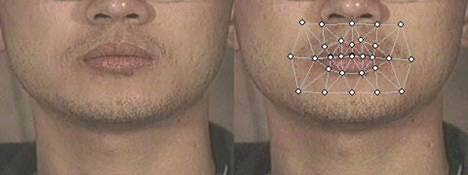
\includegraphics[height=0.75in]{mp7_image_warping_points.jpg}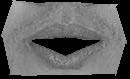
\includegraphics[height=0.75in]{mp7_image_warped.jpg}}
  \begin{align*}
    \mbox{lip\_height,width} &= \mbox{NeuralNet}\left(\mbox{audio features}\right)\\
    \mbox{out\_triangs} &= \mbox{LinearlyInterpolate}\left(\mbox{inp\_triangs,lip\_height,width}\right)\\
    \mbox{inp\_coord} &= \mbox{BaryCentric}\left(\mbox{out\_coord,inp\_triangs,out\_triangs}\right)\\
    \mbox{out\_image} &= \mbox{BilinearInterpolate}\left(\mbox{inp\_coord,inp\_image}\right)
  \end{align*}
\end{frame}


%%%%%%%%%%%%%%%%%%%%%%%%%%%%%%%%%%%%%%%%%%%%%%%%%%%%%%%%%
\section{Image Interpolation}
\setcounter{subsection}{1}

\begin{frame}
  \begin{block}{Integer Output Points}
    Now let's suppose that you've figured out the coordinate transform:
    for any given $J[y,x]$, you've figured out which pixel should be used to create it 
    ($J[y,x]=I(v,u)$).
    \lstinputlisting[language=Python]{interpolation_example.py}
  \end{block}
  \begin{block}{The Problem: Non-Integer Input Points}
    If $[x,y]$ are integers, then usually, $(u,v)$ are not integers.
  \end{block}
\end{frame}

\begin{frame}
  \frametitle{Image Interpolation}
  The function compute\_pixel performs image interpolation.
  Given the pixels of $I[n,m]$ at integer values of $m$ and $n$, it computes
  the pixel at a non-integer position $I(v,u)$ as:
  \[
  I(v,u) = \sum_m\sum_n I[n,m] h(v-n,u-m)
  \]
\end{frame}

\begin{frame}
  \frametitle{Piece-Wise Constant Interpolation}
  \begin{equation}
  I(v,u) = \sum_m\sum_n I[n,m] h(v-n,u-m)
  \label{eq:interpolation1}
  \end{equation}
  For example, suppose
  \[
  h(v,u) = \left\{\begin{array}{ll}
  1 & 0\le u<1,~~0\le v<1\\
  0 & \mbox{otherwise}
  \end{array}\right.
  \]
  Then Eq. (\ref{eq:interpolation1}) is the same as just truncating $u$
  and $v$ to the next-lower integer, and outputting that number:
  \[
  I(v,u) = I\left[\lfloor v\rfloor,\lfloor u\rfloor\right]
  \]
  where $\lfloor u\rfloor$ means ``the largest integer smaller than $u$''.
\end{frame}

\begin{frame}
  \frametitle{Example: Original Image}
  For example, let's downsample this image, and then try to recover it by image interpolation:
  \centerline{\includegraphics[width=4.5in]{exp/original.png}}
\end{frame}

\begin{frame}
  \frametitle{Example: Downsampled Image}
  Here's the downsampled image:
  \centerline{\includegraphics[width=4.5in]{exp/downsampled.png}}
\end{frame}

\begin{frame}
  \frametitle{Example: Upsampled Image} Here it is after we upsample
  it back to the original resolution (insert 3 zeros between every
  pair of nonzero columns):
  \centerline{\includegraphics[width=4.5in]{exp/upsample.png}}
\end{frame}

\begin{frame}
  \frametitle{Example: PWC Interpolation}

  Here is the piece-wise constant interpolated image:
  \centerline{\includegraphics[width=4.5in]{exp/pwc.png}}
\end{frame}

\begin{frame}
  \frametitle{Bi-Linear Interpolation}
  \[
  I(v,u) = \sum_m\sum_n I[n,m] h(v-n,u-m)
  \]
  For example, suppose
  \[
  h(v,u) = \max\left(0,(1-|u|)(1-|v|)\right)
  \]
  Then Eq. (\ref{eq:interpolation1}) is the same as piece-wise linear
  interpolation among the four nearest pixels.  This is called {\bf
    bilinear interpolation} because it's linear in two directions.
  \begin{align*}
    m &= \lfloor u\rfloor,~~~e=u-m\\
    n &= \lfloor v\rfloor,~~~f=v-m\\
    I(v,u) &= (1-e)(1-f)I[n,m]+(1-e)fI[n,m+1]\\
    &+e(1-f)I[n+1,m]+efI[n+1,m+1]
  \end{align*}
\end{frame}

\begin{frame}
  \frametitle{Example: Upsampled Image}

  Here's the upsampled image again:
  \centerline{\includegraphics[width=4.5in]{exp/upsample.png}}
\end{frame}

\begin{frame}
  \frametitle{Example: Bilinear Interpolation}

  Here it is after bilinear interpolation:
  \centerline{\includegraphics[width=4.5in]{exp/pwl.png}}
\end{frame}


\begin{frame}
  \frametitle{PWC and PWL Interpolator Kernels}

  Bilinear interpolation uses a PWL interpolation kernel, which does
  not have the abrupt discontiuity of the PWC interpolator kernel.
  \centerline{\includegraphics[width=4.5in]{exp/interpolators.png}}
\end{frame}


\begin{frame}
  \frametitle{Sinc Interpolation}
  \[
  I(v,u) = \sum_m\sum_n I[n,m] h(v-n,u-m)
  \]
  For example, suppose
  \[
  h(v,u) = \mbox{sinc}(\pi u)\mbox{sinc}(\pi v)
  \]
  Then Eq. (\ref{eq:interpolation1}) is an ideal band-limited sinc interpolation.
  It guarantees that the continuous-space image, $I(v,u)$, is exactly a band-limited
  D/A reconstruction of the digital image $I[n,m]$.
\end{frame}

\begin{frame}
  \frametitle{Sinc Interpolation}

  Here is the cat after sinc interpolation:
  \centerline{\includegraphics[width=4.5in]{exp/sincinterp.png}}
\end{frame}

\begin{frame}
  \frametitle{Original, Upsampled, and Sinc-Interpolated Spectra}

  Here are the magnitude Fourier transforms of the original,
  upsampled, and sinc-interpolated cat.
  
  \centerline{\includegraphics[width=4.5in]{exp/downsampled_spectra.png}}
\end{frame}

\begin{frame}
  \frametitle{Original, Upsampled, and Sinc-Interpolated Spectra}

  Here are the magnitude Fourier transforms of the original,
  upsampled, and sinc-interpolated cat.

  \centerline{
    \begin{tikzpicture}
      \node[inner sep=0pt](spectra) at (0,1.5) {
        \includegraphics[height=5cm]{exp/downsampled_spectra.png}};
      \node[inner sep=0pt](orig) at (4.5,2.8) {
        \includegraphics[height=1.5cm]{exp/original.png}};
      \node[inner sep=0pt](up) at (4.5,1.5) {
        \includegraphics[height=1.5cm]{exp/upsample.png}};
      \node[inner sep=0pt](sinc)  at (4.5,0.2) {
        \includegraphics[height=1.5cm]{exp/sincinterp.png}};
  \end{tikzpicture}}
  \vspace*{-0.5cm}
  \begin{itemize}
  \item The zeros in the upsampled cat correspond to aliasing in its spectrum.
  \item The ringing in the sinc-interpolated cat corresponds to the
    sharp cutoff, at pi/4, of its spectrum.
  \end{itemize}
\end{frame}



%%%%%%%%%%%%%%%%%%%%%%%%%%%%%%%%%%%%%%%%%%%%%%%%%%%%%%%%%
\section{Deep Voxel Flow}
\setcounter{subsection}{1}

\begin{frame}
  \frametitle{\href{https://openaccess.thecvf.com/content_ICCV_2017/papers/Liu_Video_Frame_Synthesis_ICCV_2017_paper.pdf}{Video Frame Synthesis Using Deep Voxel Flow}\\\begin{small}Liu et al., ICCV 2017\end{small}}
  \centerline{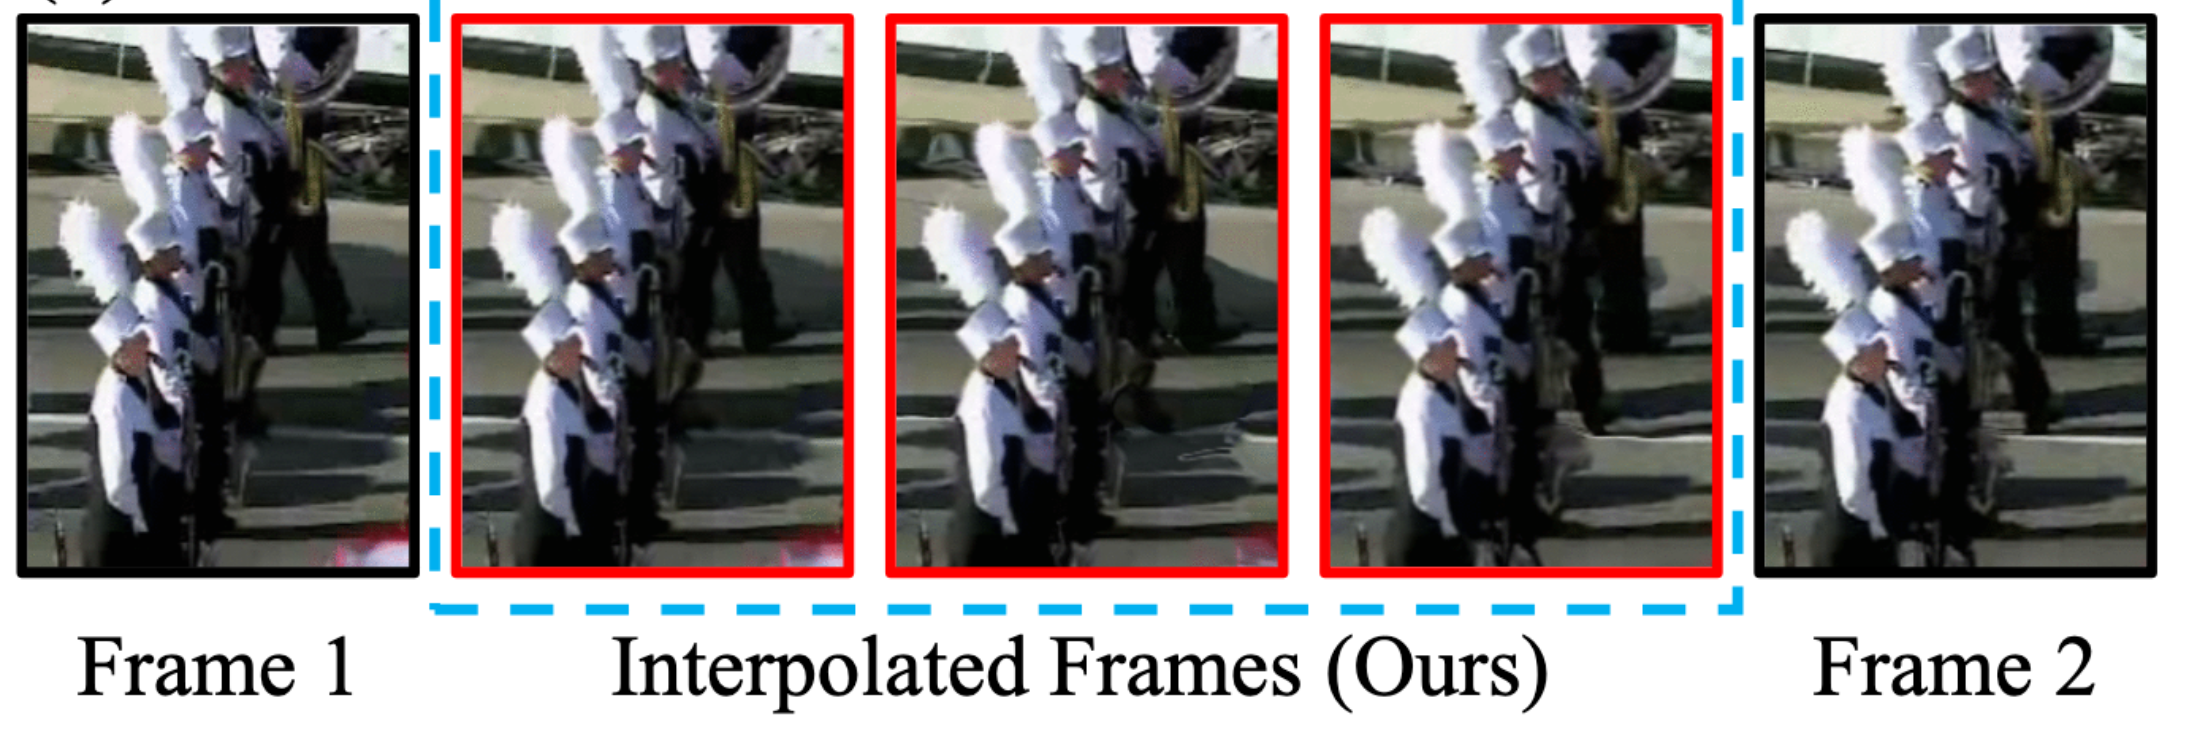
\includegraphics[width=4.5in]{figs/liu17iccv4a.png}}
  \begin{small}Image (c) ICCV and the authors\end{small}
\end{frame}

\begin{frame}
  \frametitle{\href{https://openaccess.thecvf.com/content_ICCV_2017/papers/Liu_Video_Frame_Synthesis_ICCV_2017_paper.pdf}{Video Frame Synthesis Using Deep Voxel Flow}\\\begin{small}Liu et al., ICCV 2017\end{small}}

  \begin{itemize}
  \item Objective: Given video frames at times $0$ and $1$, generate
    missing frame at time $t\in(0,1)$.
  \item Voxel Flow: Generated frame is made by copying pixels from frames $0$ and $1$, with
    some shift in position, $(\Delta x,\Delta y)$.
  \item The coordinate shift $(\Delta x,\Delta y)$ is (almost) a {\bf piece-wise affine} function
    of $(x,y)$, so it is (almost) equivalent to a  mapping based on Barycentric coordinates---but
    without ever explicitly choosing the triangle locations.
  \item When $(x-\Delta x,y-\Delta y)$  are non-integer, the input pixels are
    constructed using {\bf bilinear interpolation}.
  \end{itemize}
\end{frame}

\begin{frame}
  \frametitle{Voxel Flow}

  The generated frame, $\mathbf{\hat{Y}}(y,x,t)$, is generated as a
  linear convex interpolation between selected pixels of the two
  reference images, $\mathbf{X}(y,x,0)$ and $\mathbf{X}(y,x,1)$:
  \begin{displaymath}
    \mathbf{\hat{Y}}(y,x,t)=
    \left(1-\Delta t\right)\mathbf{X}\left(y-\Delta y,x-\Delta x,0\right)+
    \Delta t\mathbf{X}\left(y+\Delta y,x+\Delta x,1\right)
  \end{displaymath}
  where $\Delta t\in(0,1)$.
\end{frame}

\begin{frame}
  \frametitle{Piece-Wise (Nearly) Affine}

  The voxel flow field is generated as
  \begin{displaymath}
    \mathbf{F}=(\Delta x,\Delta y,\Delta t)={\mathcal H}\left(\mathbf{X};\theta\right)
  \end{displaymath}
  where ${\mathcal H}\left(\mathbf{X};\theta\right)$ uses:
  \begin{itemize}
  \item A series of CNN layers with ReLU nonlinearity, to compute a
    piece-wise affine function of $\mathbf{X}$, then
  \item A final layer with a $\tanh$ nonlinearity, squashing the output
    to the range $\Delta x\in\left(-1,1\right)$,
    $\Delta y\in\left(-1,1\right)$.
  \end{itemize}
\end{frame}

\begin{frame}
  \frametitle{Piece-Wise (Nearly) Affine}

  \centerline{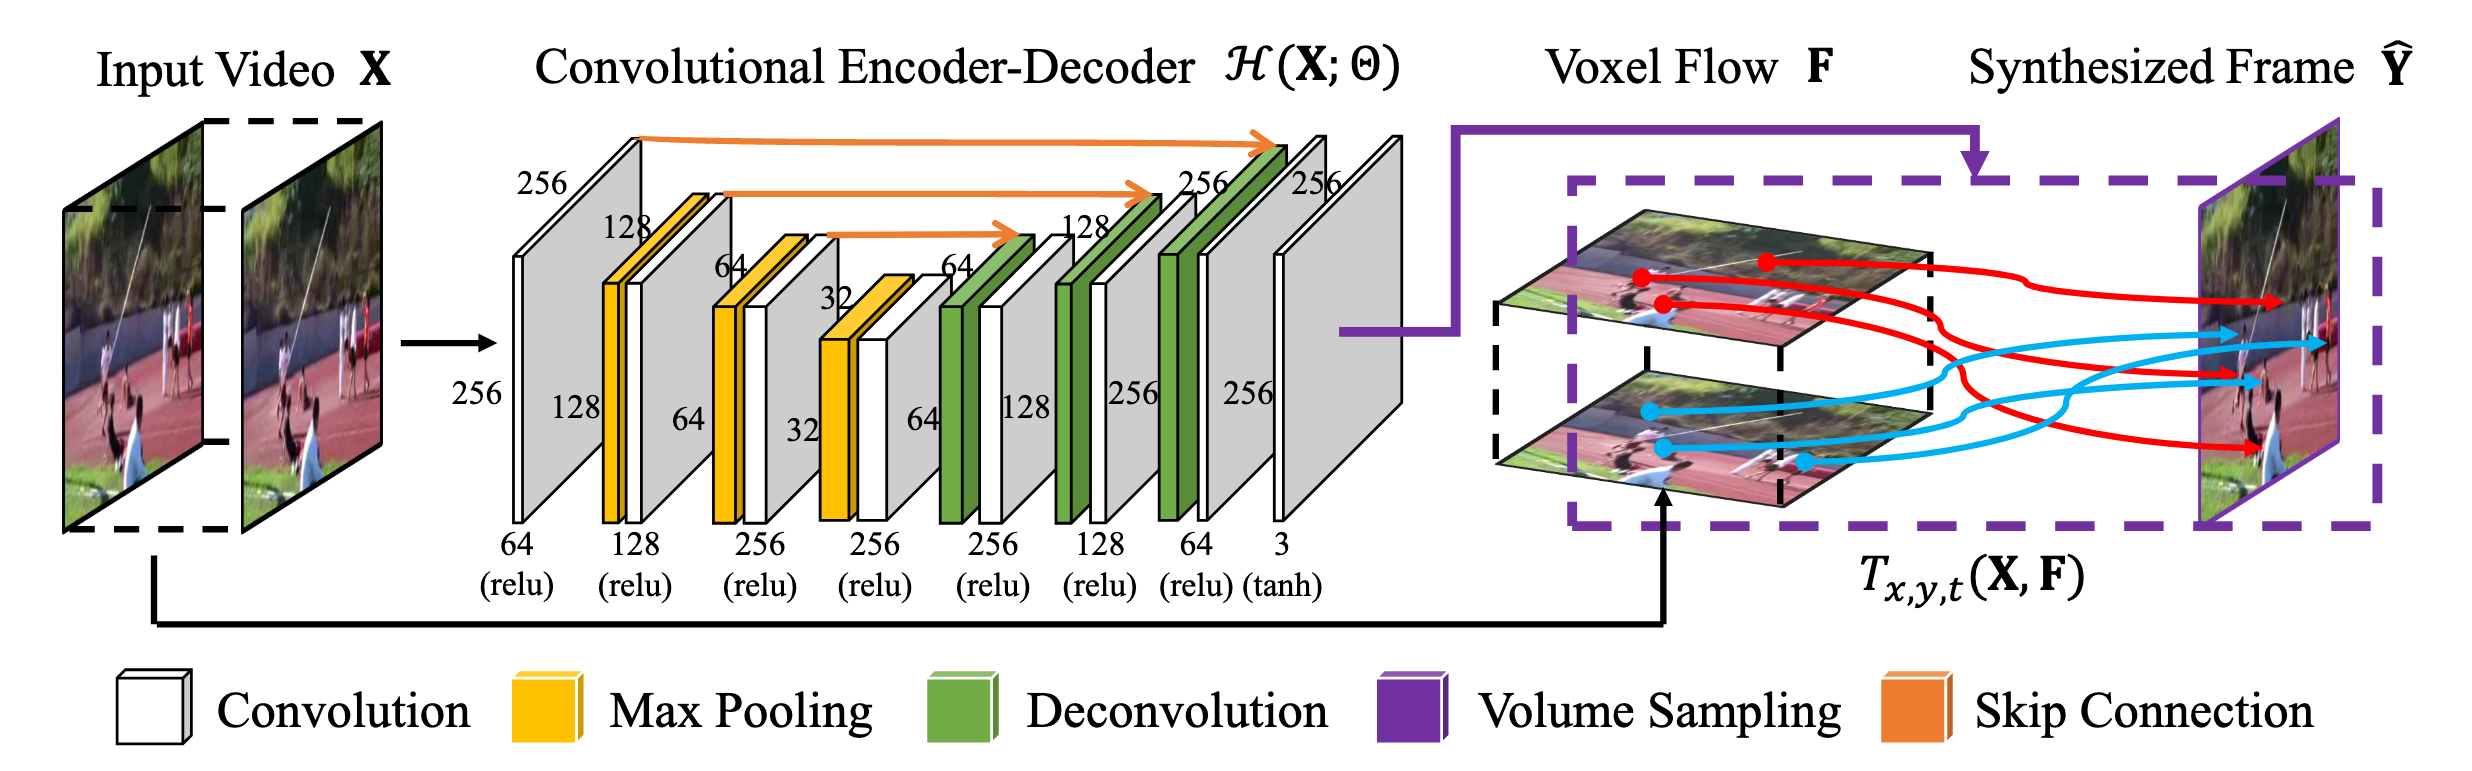
\includegraphics[width=4.5in]{figs/liu17iccv1.png}}
  \begin{small}Image (c) ICCV and the authors\end{small}
\end{frame}

\begin{frame}
  \frametitle{Bilinear Interpolation}

  The reference pixels, $\left(y-\Delta y,x-\Delta x\right)$ and
  $\left(y+\Delta y,x+\Delta x\right)$, are usually not integers, so
  they are constructed using bilinear interpolation:
  \begin{displaymath}
    \mathbf{\hat{Y}}(y,x,t) =
    \sum_{i,j,k\in\left\{0,1\right\}}\mathbf{W}^{ijk}\mathbf{X}(\mathbf{V}^{ijk}),
  \end{displaymath}
  where:
  \begin{align*}
    \mathbf{V}^{000}&=\left(\lfloor x-\Delta x\rfloor,\lfloor y-\Delta y\rfloor,0\right)\\
    \mathbf{V}^{100}&=\left(\lceil x-\Delta x\rceil,\lfloor y-\Delta y\rfloor,0\right)\\
    &\vdots\\
    \mathbf{V}^{111}&=\left(\lceil x+\Delta x\rceil,\lceil y+\Delta y\rceil,1\right)
  \end{align*}
  and the weights $\mathbf{W}^{ijk}$ are constructed according to bilinear interpolation.
\end{frame}
    
\begin{frame}
  \frametitle{Differentiable}

  Because bilinear interpolation is a piece-wise linear function of
  $\Delta x$ and $\Delta y$, the error can be differentiated
  w.r.t. those parameters.  From the original paper:
  \centerline{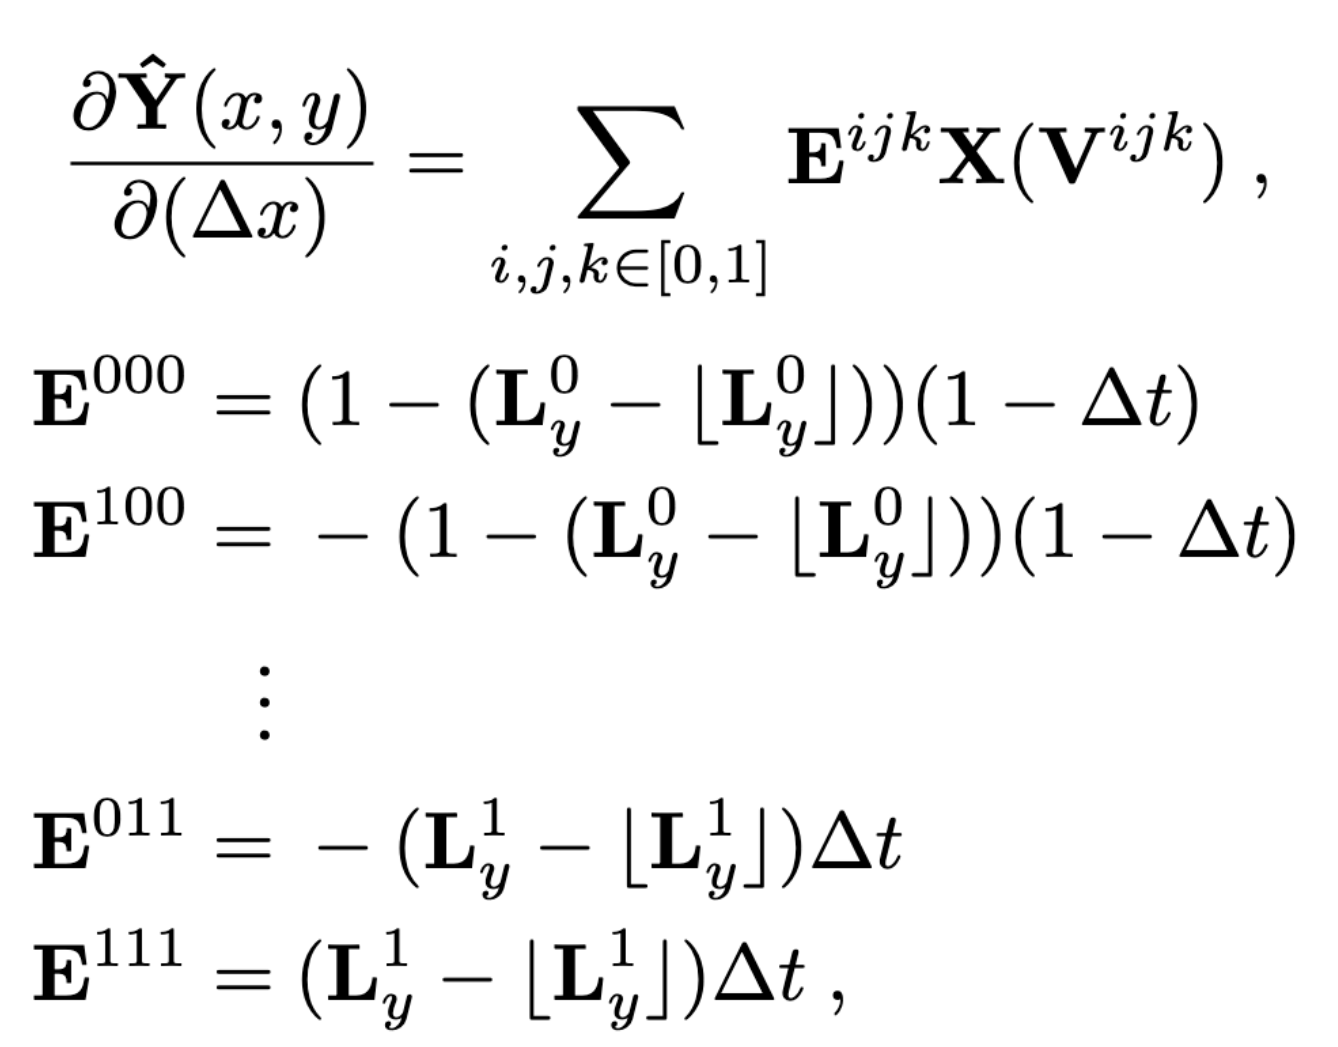
\includegraphics[height=2in]{figs/liu17iccv7.png}}
\end{frame}
    

%%%%%%%%%%%%%%%%%%%%%%%%%%%%%%%%%%%%%%%%%%%%%%%%%%%%%%%%%
\section{Conclusion}
\setcounter{subsection}{1}

\begin{frame}
  \frametitle{How to Make a Talking Head}
  \centerline{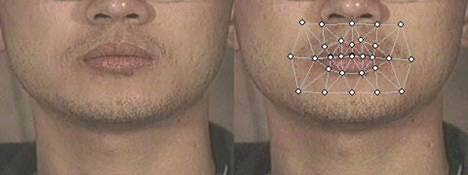
\includegraphics[height=0.75in]{mp7_image_warping_points.jpg}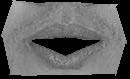
\includegraphics[height=0.75in]{mp7_image_warped.jpg}}
  \begin{align*}
    \mbox{lip\_height,width} &= \mbox{NeuralNet}\left(\mbox{audio features}\right)\\
    \mbox{out\_triangs} &= \mbox{LinearlyInterpolate}\left(\mbox{inp\_triangs,lip\_height,width}\right)\\
    \mbox{inp\_coord} &= \mbox{BaryCentric}\left(\mbox{out\_coord,inp\_triangs,out\_triangs}\right)\\
    \mbox{out\_image} &= \mbox{BilinearInterpolate}\left(\mbox{inp\_coord,inp\_image}\right)
  \end{align*}
\end{frame}

\begin{frame}
  \frametitle{Barycentric Coordinates}

  \begin{itemize}
  \item For each of the triangles, find $\vec\lambda=X_k^{-1}\vec{x}$.
  \item Choose the triangle for which all of the $\lambda$ coefficients
    are $0\le\lambda\le 1$.
  \item Find $\vec{u}=U_k\vec\lambda$.
  \item Estimate $I(v,u)$ using bilinear interpolation.
    \[
    I(v,u) = \sum_m\sum_n I[n,m] h(v-n,u-m)
    \]    
  \item Set $J[y,x]=I(v,u)$.
  \end{itemize}
\end{frame}

\begin{frame}
  \frametitle{Deep Voxel Flow: PWL$\Rightarrow$End-to-end differentiable}

  \centerline{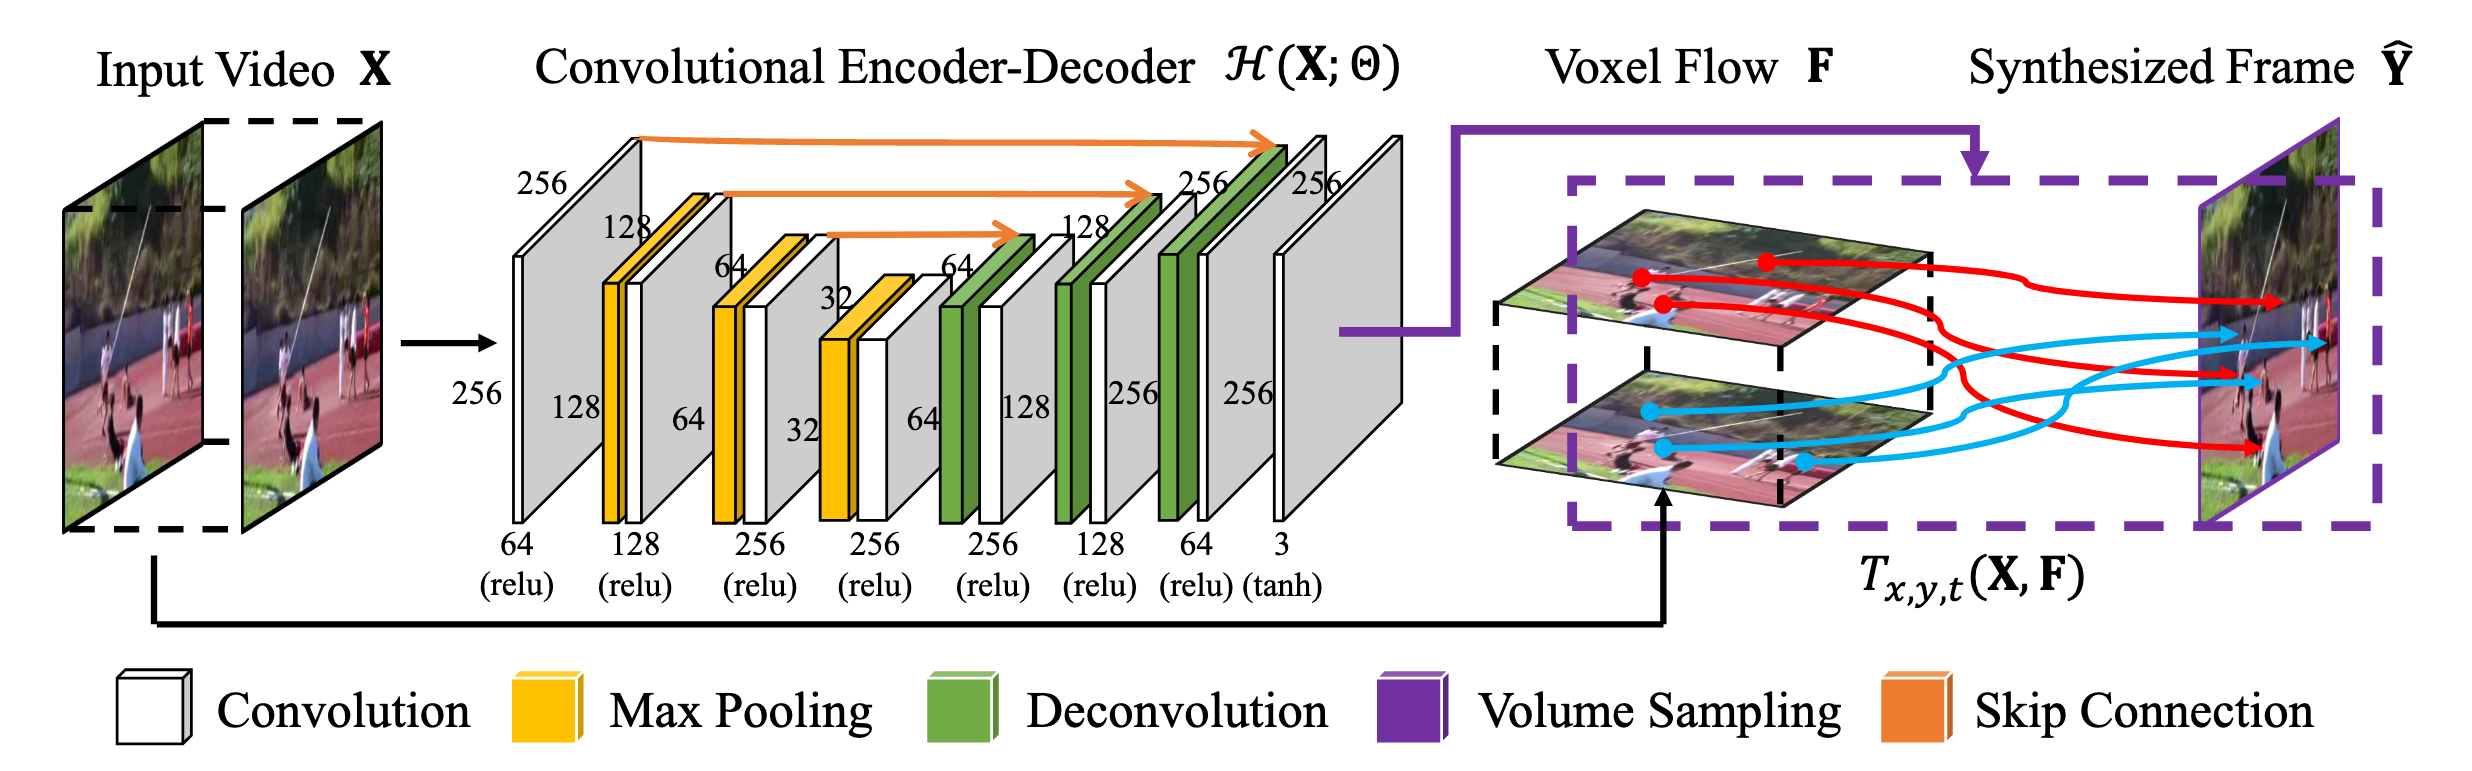
\includegraphics[width=4.5in]{figs/liu17iccv1.png}}
  \begin{small}Image (c) ICCV and the authors\end{small}
\end{frame}

\end{document}

